\chapter{Testowania modeli}
Wygenerowałem losowe wartości wymuszeń z przedziału $\begin{bmatrix} -45 & 45 \end{bmatrix}$. Na potrzeby testów przyjąłem stałą wartość zakłócenia, tj.

\begin{equation}
F_D = F_{D0}
\end{equation} 

\noindent gdzie $F_{D0}$ - wartość z punktu pracy
\begin{lstlisting}[style=Matlab-editor]
for i = 1:5
U = [repelem((rand(1, obiekt.kk/250) * 90 - 45), 250); 
	zeros(1, obiekt.kk)];
    
hammerstein.testLinearModel(U, a, b, obiekt.delay, obiekt.kk,...
			obiekt.Tp, @(x, y) obiekt.rk4(x, y), i);
hammerstein.testNonlinearModel(U, a, b, obiekt.delay, obiekt.kk,...
			obiekt.Tp, @(x, y) obiekt.rk4(x, y), i);
    
wiener.testLinearModel(U, a, b, obiekt.delay, obiekt.kk,...
			obiekt.Tp, @(x, y) obiekt.rk4(x, y), i);
wiener.testNonlinearModel(U, a, b, obiekt.delay, obiekt.kk,...
			obiekt.Tp, @(x, y) obiekt.rk4(x, y), i);
end
\end{lstlisting}

\noindent Wykonano pięć takich testów. Udało się bez utraty dokładności zbudować model obiektu z wykorzystaniem hiperbolicznych następników w modelach Takagi - Sugeno. Rezultaty przedstawiono poniżej.

*W legendach obok opisu danego przebiegu zamieściłem wartość wskaźnika jakości w postaci błędu kwadratowego, tj. 
\begin{equation}
E = \sum_{i=1}^{N} (y(i) - y_{mod}(i))^2
\end{equation} 

\noindent gdzie $y$ - wartość otrzymana dla algorytmu Rungego-Kutty 4 rzędu

\newpage

\newgeometry{left=1mm, right=1mm, top=25mm, bottom=25mm} 

\begin{figure}[b!]
\centering
\begin{subfigure}[b]{0.49\paperwidth}
\centering
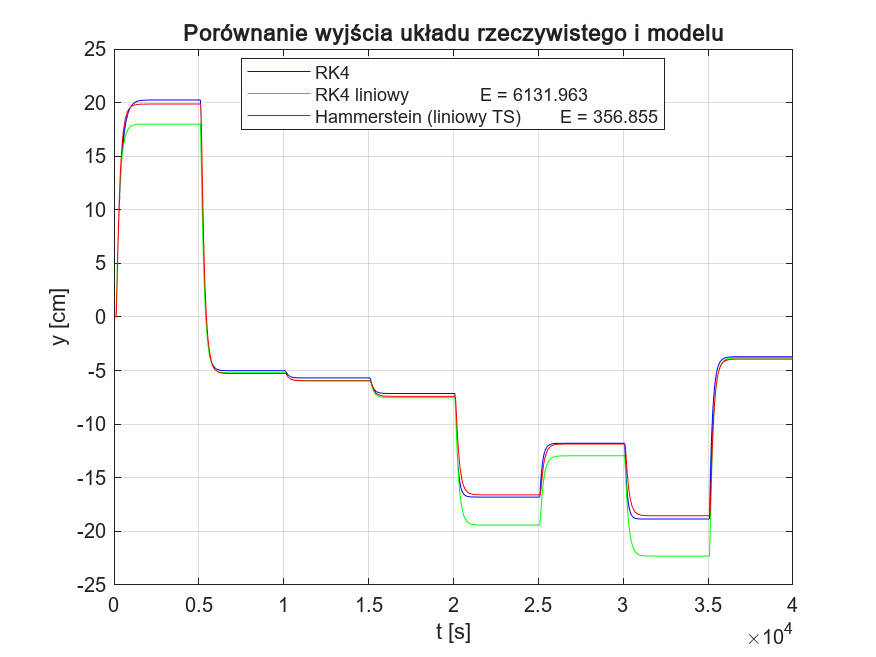
\includegraphics[width=\linewidth]{pictures/HammersteinLinearModel_1}
\caption{Hammerstein - następniki liniowe.}
\end{subfigure}
\hfill
\begin{subfigure}[b]{0.49\paperwidth}
\centering
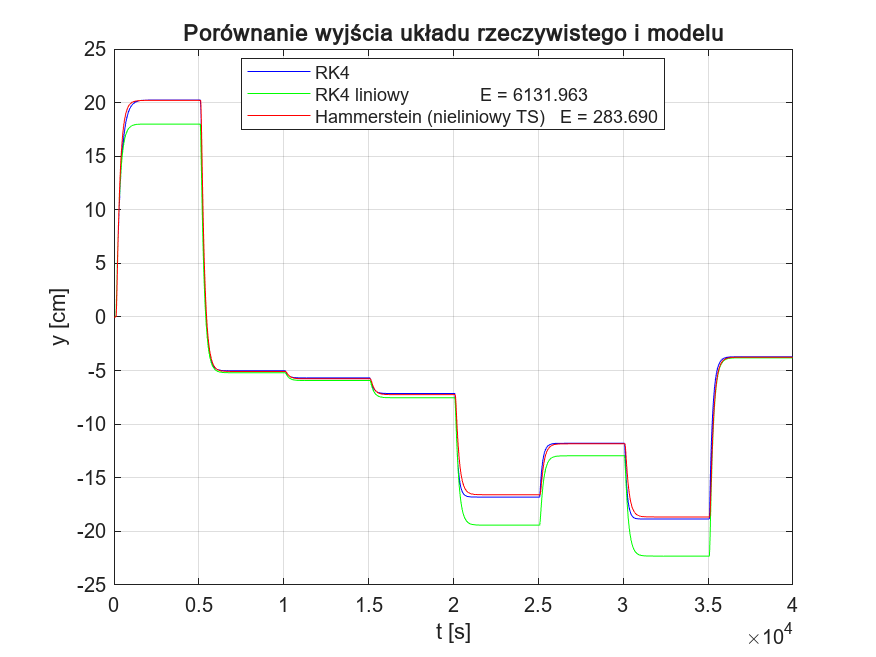
\includegraphics[width=\linewidth]{pictures/HammersteinNonlinearModel_1}
\caption{Hammerstein -  następniki nieliniowe.}
\end{subfigure}
    
\vspace{0.5cm} % Dystans pionowy między rzędami

\begin{subfigure}[b]{0.49\paperwidth}
\centering
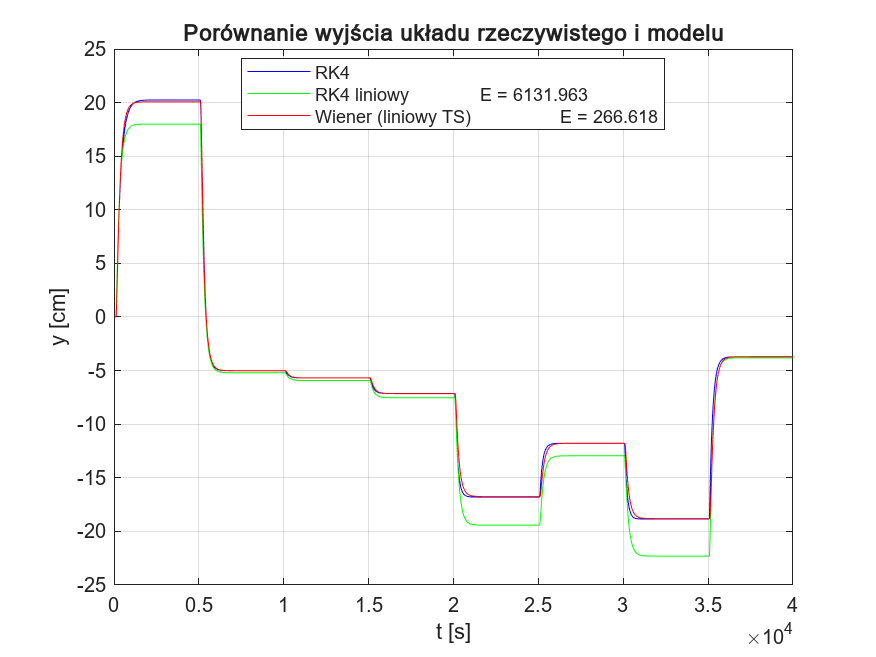
\includegraphics[width=\linewidth]{pictures/WienerLinearModel_1}
\caption{Wiener - następniki liniowe.}
\end{subfigure}
\hfill
\begin{subfigure}[b]{0.49\paperwidth}
\centering
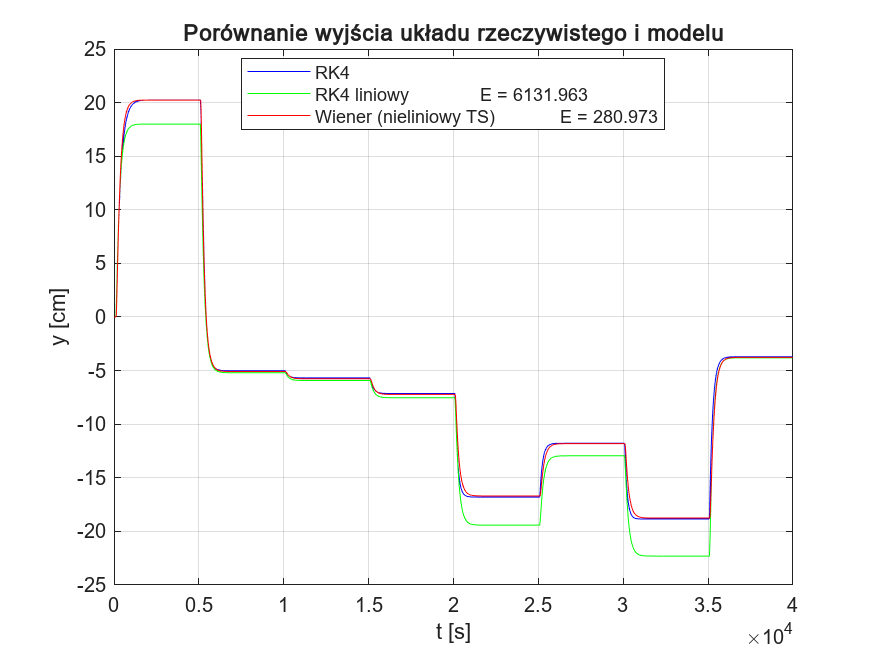
\includegraphics[width=\linewidth]{pictures/WienerNonlinearModel_1}
\caption{Wiener - następniki nieliniowe.}
\end{subfigure}

\caption{Pierwsza seria modeli.}
\end{figure}

\newpage

\begin{figure}[b!]
\centering
\begin{subfigure}[b]{0.49\paperwidth}
\centering
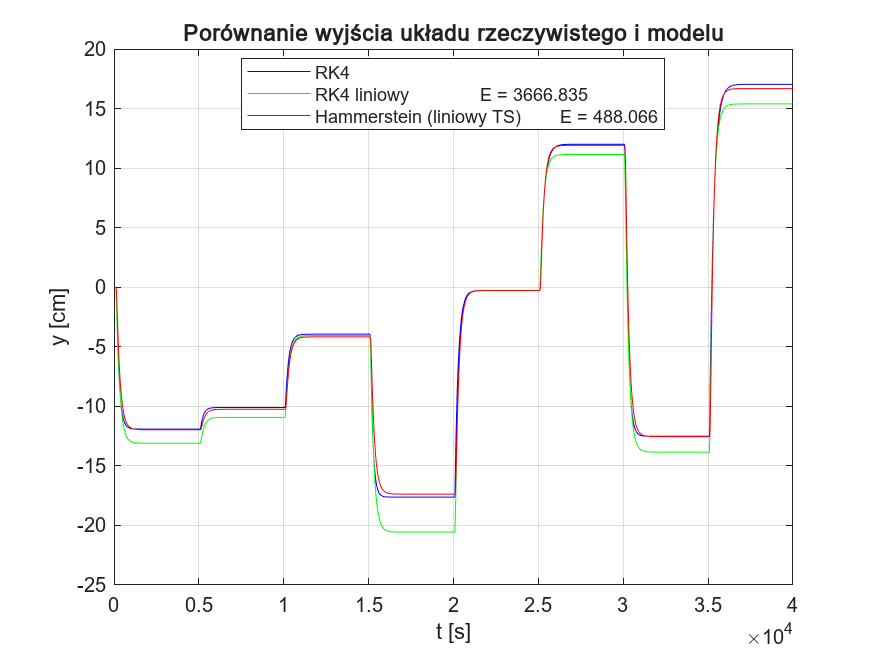
\includegraphics[width=\linewidth]{pictures/HammersteinLinearModel_2}
\caption{Hammerstein - następniki liniowe.}
\end{subfigure}
\hfill
\begin{subfigure}[b]{0.49\paperwidth}
\centering
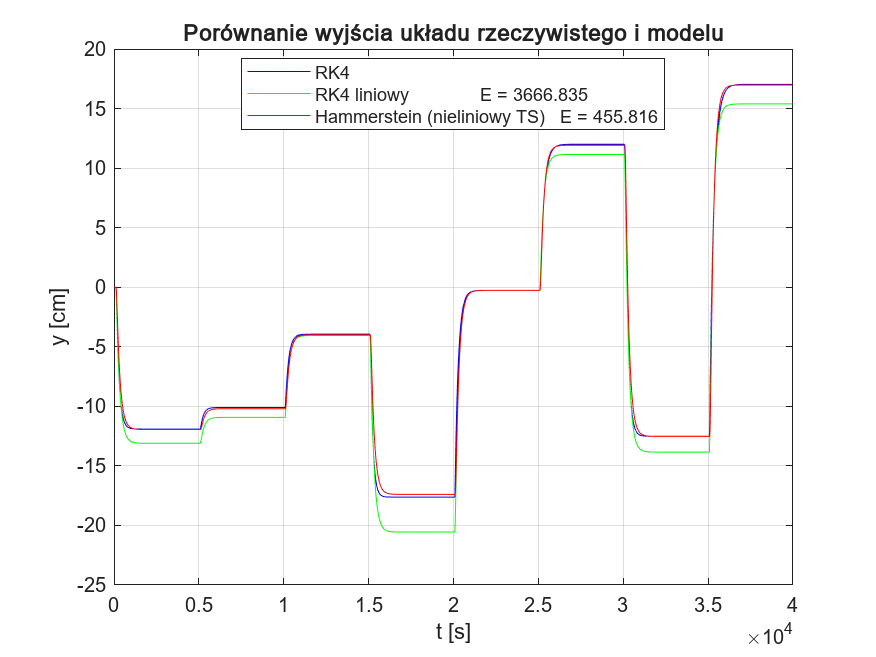
\includegraphics[width=\linewidth]{pictures/HammersteinNonlinearModel_2}
\caption{Hammerstein - następniki nieliniowe.}
\end{subfigure}
    
\vspace{0.5cm} % Dystans pionowy między rzędami

\begin{subfigure}[b]{0.49\paperwidth}
\centering
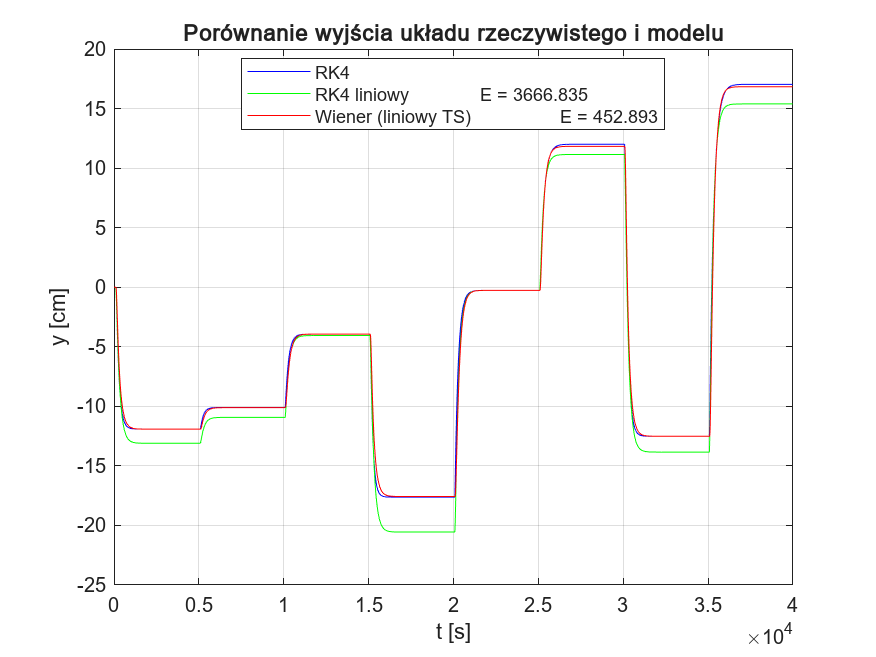
\includegraphics[width=\linewidth]{pictures/WienerLinearModel_2}
\caption{Wiener - następniki liniowe.}
\end{subfigure}
\hfill
\begin{subfigure}[b]{0.49\paperwidth}
\centering
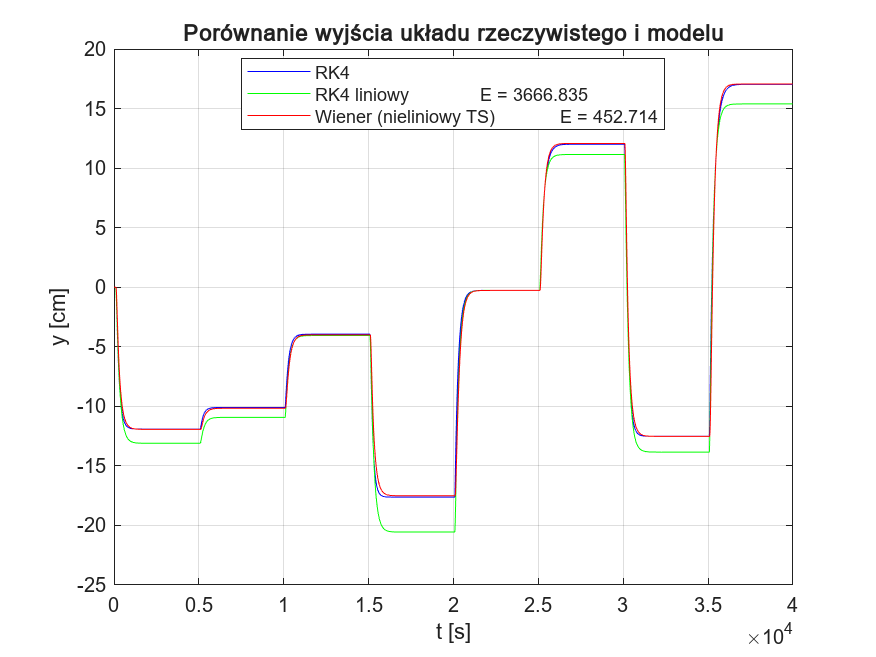
\includegraphics[width=\linewidth]{pictures/WienerNonlinearModel_2}
\caption{Wiener - następniki nieliniowe.}
\end{subfigure}

\caption{Druga seria modeli.}
\end{figure}

\newpage

\begin{figure}[b!]
\centering
\begin{subfigure}[b]{0.49\paperwidth}
\centering
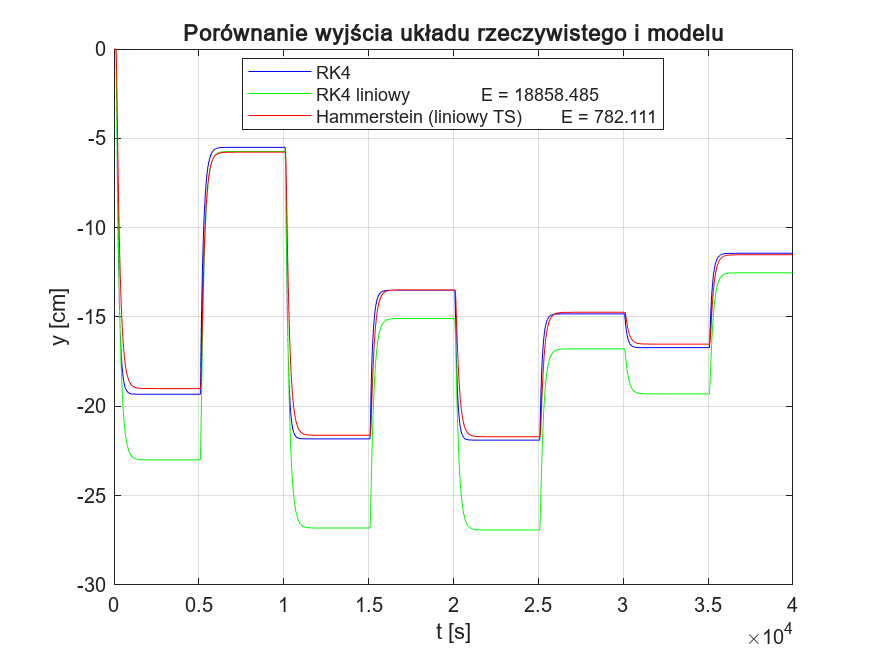
\includegraphics[width=\linewidth]{pictures/HammersteinLinearModel_3}
\caption{Hammerstein - następniki liniowe.}
\end{subfigure}
\hfill
\begin{subfigure}[b]{0.49\paperwidth}
\centering
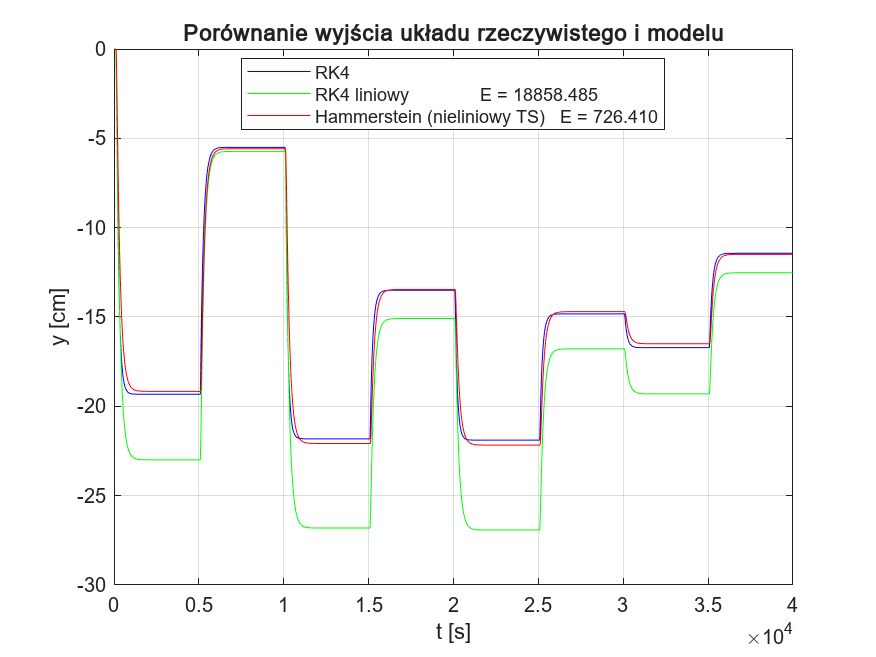
\includegraphics[width=\linewidth]{pictures/HammersteinNonlinearModel_3}
\caption{Hammerstein - następniki nieliniowe.}
\end{subfigure}
    
\vspace{0.5cm} % Dystans pionowy między rzędami

\begin{subfigure}[b]{0.49\paperwidth}
\centering
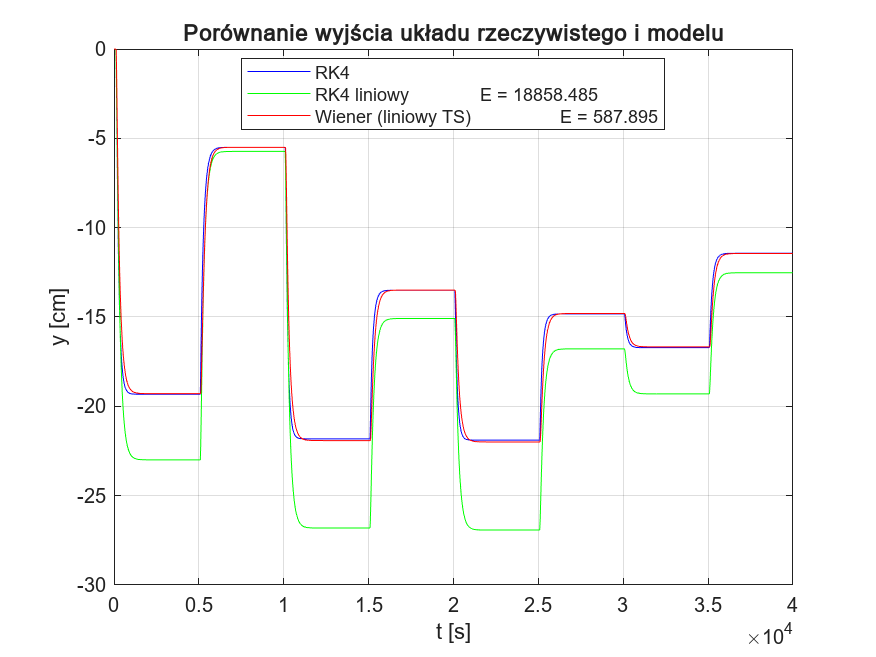
\includegraphics[width=\linewidth]{pictures/WienerLinearModel_3}
\caption{Wiener - następniki liniowe.}
\end{subfigure}
\hfill
\begin{subfigure}[b]{0.49\paperwidth}
\centering
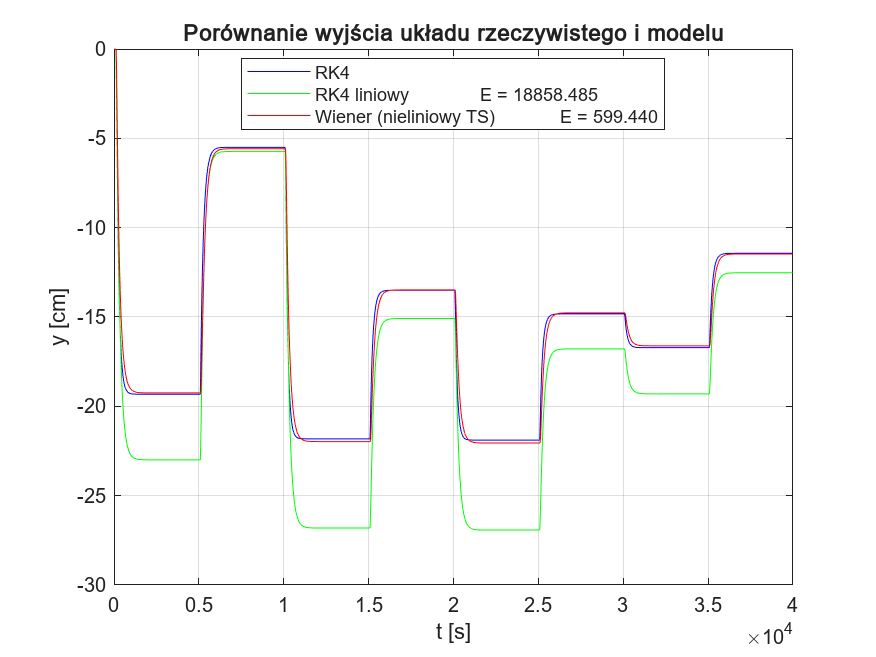
\includegraphics[width=\linewidth]{pictures/WienerNonlinearModel_3}
\caption{Wiener - następniki nieliniowe.}
\end{subfigure}

\caption{Trzecia seria modeli.}
\end{figure}

\newpage

\begin{figure}[b!]
\centering
\begin{subfigure}[b]{0.49\paperwidth}
\centering
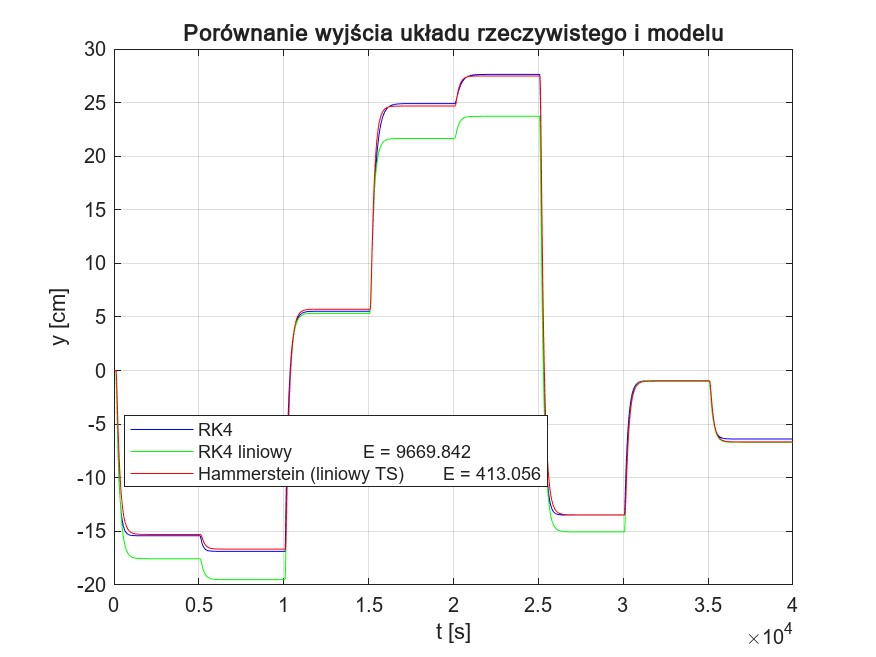
\includegraphics[width=\linewidth]{pictures/HammersteinLinearModel_4}
\caption{Hammerstein - następniki liniowe.}
\end{subfigure}
\hfill
\begin{subfigure}[b]{0.49\paperwidth}
\centering
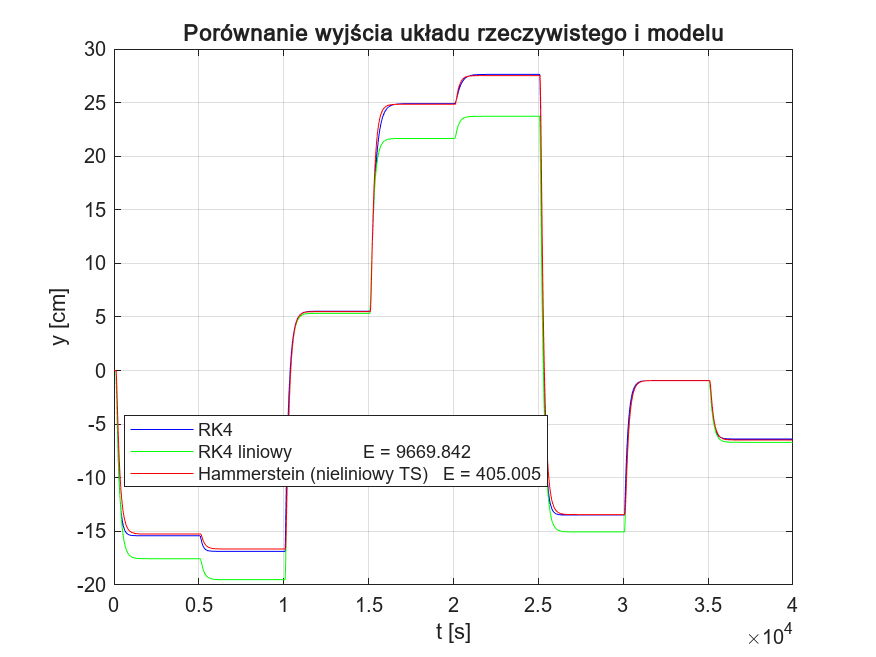
\includegraphics[width=\linewidth]{pictures/HammersteinNonlinearModel_4}
\caption{Hammerstein - następniki nieliniowe.}
\end{subfigure}
    
\vspace{0.5cm} % Dystans pionowy między rzędami

\begin{subfigure}[b]{0.49\paperwidth}
\centering
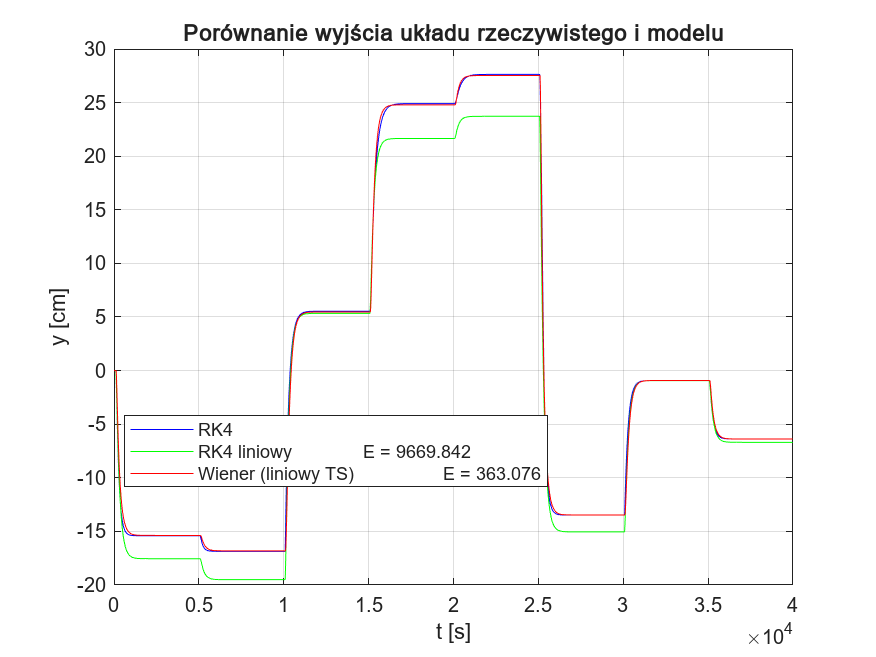
\includegraphics[width=\linewidth]{pictures/WienerLinearModel_4}
\caption{Wiener - następniki liniowe.}
\end{subfigure}
\hfill
\begin{subfigure}[b]{0.49\paperwidth}
\centering
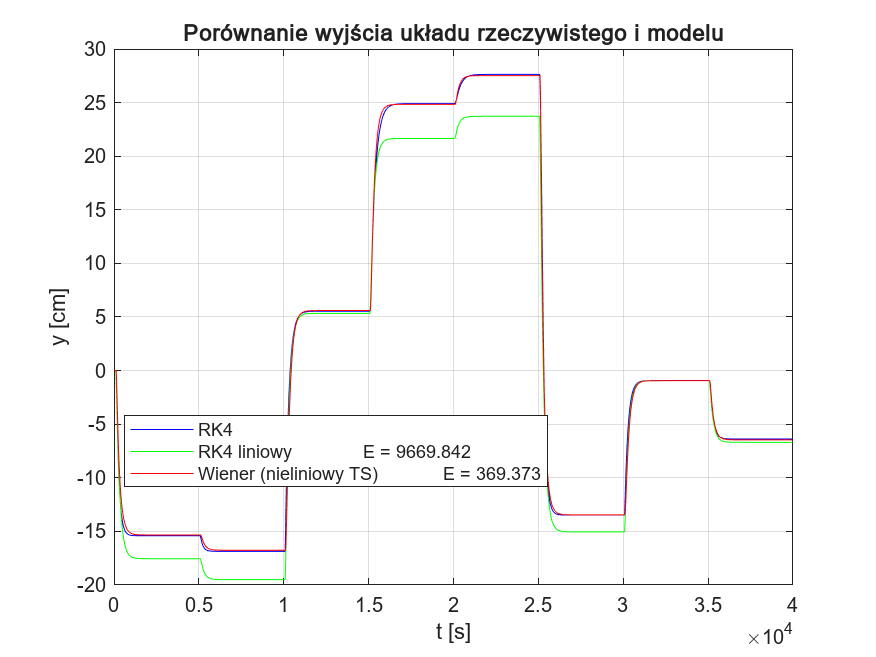
\includegraphics[width=\linewidth]{pictures/WienerNonlinearModel_4}
\caption{Wiener - następniki nieliniowe.}
\end{subfigure}

\caption{Czwarta seria modeli.}
\end{figure}

\newpage

\begin{figure}[b!]
\centering
\begin{subfigure}[b]{0.49\paperwidth}
\centering
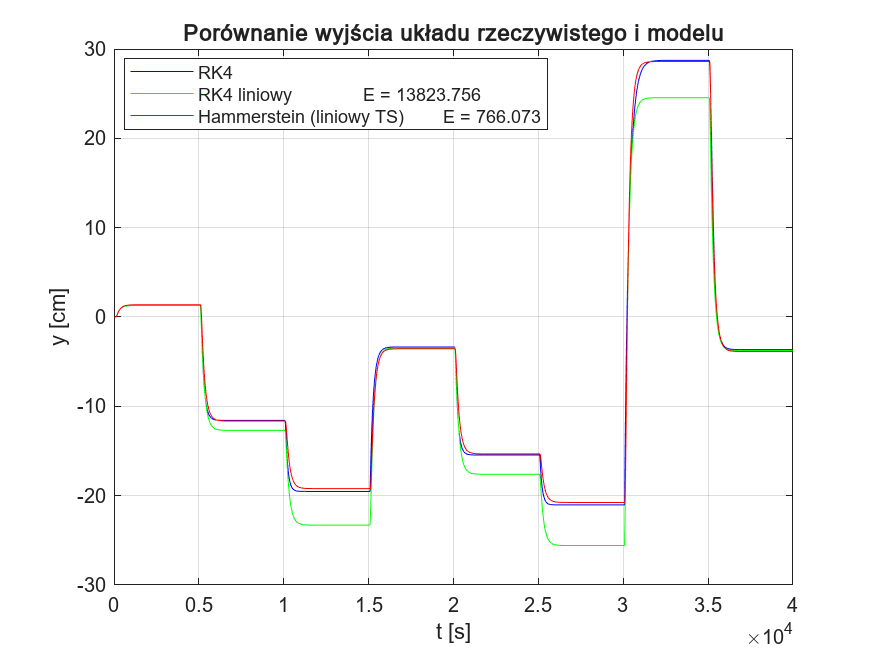
\includegraphics[width=\linewidth]{pictures/HammersteinLinearModel_5}
\caption{Hammerstein - następniki liniowe.}
\end{subfigure}
\hfill
\begin{subfigure}[b]{0.49\paperwidth}
\centering
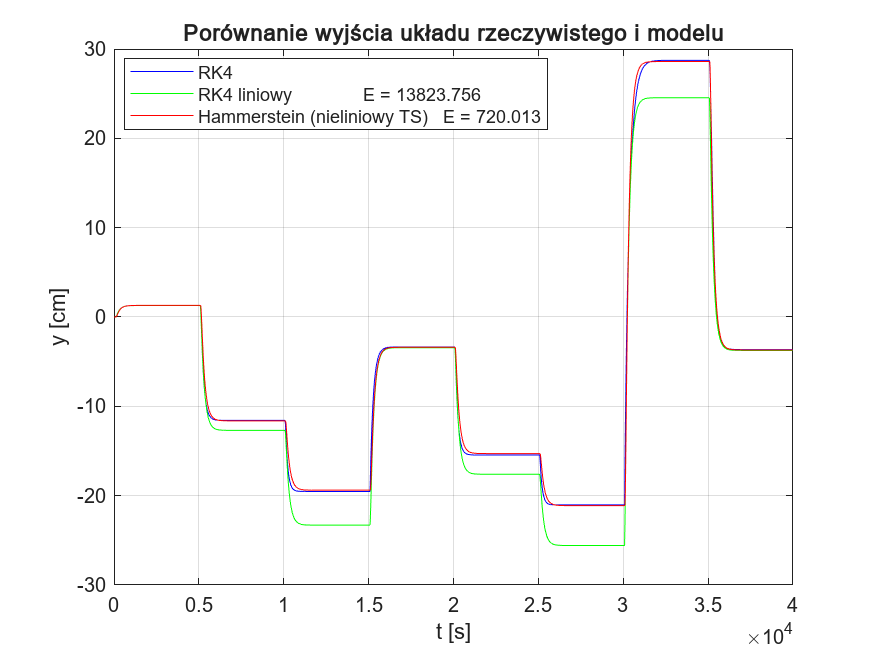
\includegraphics[width=\linewidth]{pictures/HammersteinNonlinearModel_5}
\caption{Hammerstein - następniki nieliniowe.}
\end{subfigure}
    
\vspace{0.5cm} % Dystans pionowy między rzędami

\begin{subfigure}[b]{0.49\paperwidth}
\centering
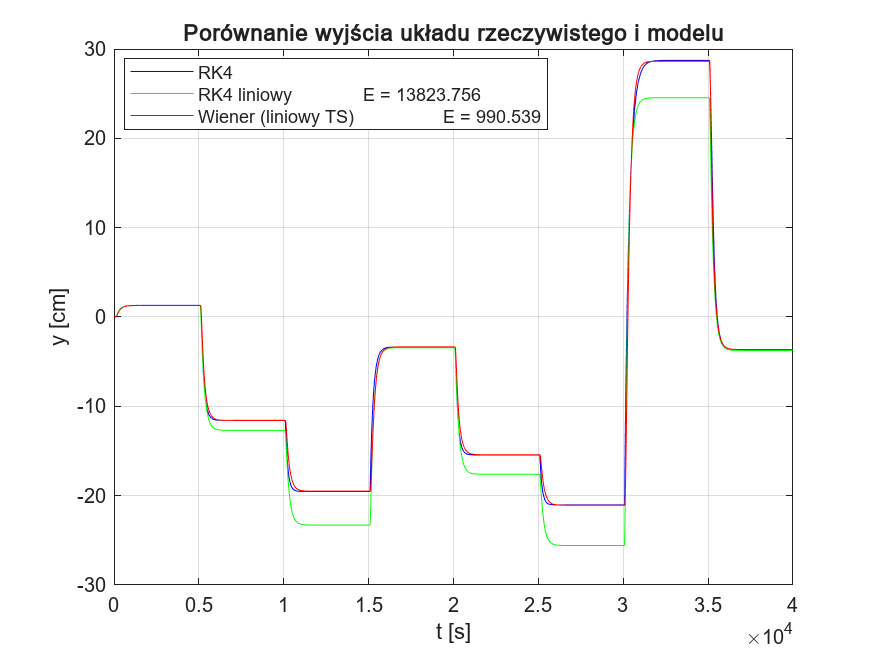
\includegraphics[width=\linewidth]{pictures/WienerLinearModel_5}
\caption{Wiener - następniki liniowe.}
\end{subfigure}
\hfill
\begin{subfigure}[b]{0.49\paperwidth}
\centering
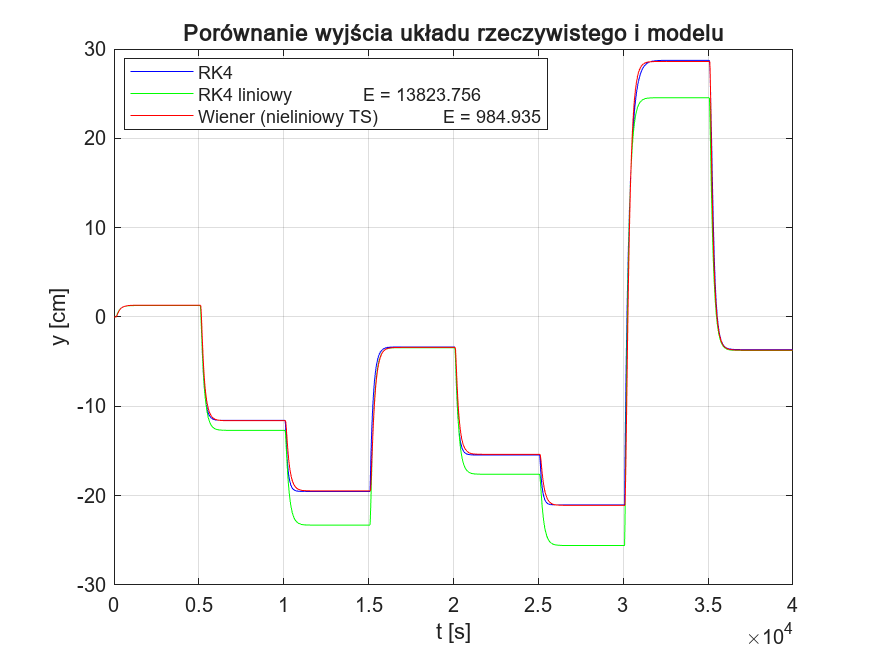
\includegraphics[width=\linewidth]{pictures/WienerNonlinearModel_5}
\caption{Wiener - następniki nieliniowe.}
\end{subfigure}

\caption{Piąta seria modeli.}
\end{figure}

\restoregeometry 
\newpage